\documentclass[conference]{IEEEtran}
\IEEEoverridecommandlockouts
\usepackage{cite}
\usepackage{amsmath,amssymb,amsfonts}
\usepackage{graphicx}
\usepackage{booktabs}
\usepackage{multirow}
\usepackage{xcolor}
\usepackage[hidelinks]{hyperref}
\usepackage{url}

% Numbers that come from the learned-vs-geometric ablation (filled in from results/tselgeom_*.jsonl)
\newcommand{\GeomSummary}{under the same lookahead lowered success after one touch from 95.4\% to 93.8\% (-1.7 points, 95\% CI [-4.6, +1.2], McNemar $p=0.424$)}
\newcommand{\GeomDiffShort}{+1.7 points}
\newcommand{\GeomResultsParagraph}{With the geometric tolerance in place of $f_\phi$ (\Geom), success after one touch was 93.8\%, against 95.4\% for \Ours{} (paired difference +1.7 points, 95\% CI [-1.2, +4.6]; discordant layouts 9 vs.\ 5; McNemar $p=0.424$). By visible length, \Ours{} minus \Geom{} was +1.7 [-3.3, +6.7] at 10\,mm, +0.0 [-5.0, +5.0] at 15\,mm, +3.3 [-3.3, +10.0] at 20\,mm, +1.7 [-5.0, +8.3] at 25\,mm. After two touches, success was 95.0\% versus 94.2\% (+0.8 [-2.5, +4.6], $p=0.815$). The median spread of the body front edge after one touch was 2.7\,mm (\Ours) and 2.7\,mm (\Geom).}


\newcommand{\Ours}{Ours}
\newcommand{\Unc}{MaxUnc}
\newcommand{\Rand}{Random}
\newcommand{\Geom}{Ours-Geom}

\begin{document}

\title{Where to Touch to Grasp a Partially Occluded Part:\\Touching Where the Grasp Success Probability Rises Most}

\author{\IEEEauthorblockN{AUTHOR NAME}
\IEEEauthorblockA{Independent Researcher\\
Japan\\
EMAIL}}

\maketitle

\begin{abstract}
A small part stored under a shelf is often visible only at its front: the shelf board hides the rest from the robot's head camera, and the hidden part of the shape decides where the part can be pinched. We propose to resolve this with a single light touch chosen for the grasp, not for the shape. Shape candidates (particles) are initialized from segmentation and depth, and a small neural network trained on 8,000 physics-randomized simulated grasps predicts the grasp success of each candidate at each grasp point. The robot touches the point that maximizes the expected best grasp success after the touch, i.e., where either outcome, hit or miss, makes it clear where to grasp next. On 240 paired layouts with a Unitree G1 humanoid and a three-finger hand in MuJoCo, grasp success after one touch was 95.4\% with our rule, against 88.8\% when touching where shape uncertainty is largest and 88.8\% for random touches (+6.7 points, 95\% CI [+2.1, +11.3], McNemar $p=0.005$). The gap grew to +15.0 points when only 10\,mm of the part was visible. With a hand-measured geometric tolerance in place of the learned model, the same lookahead reached \GeomSummary: the gain comes mainly from choosing the touch for the grasp, not from learning. Grasping without touching succeeded in 72.5\% of layouts, and failed grasps moved the part by more than 10\,mm in most cases. A rule that stops touching once the predicted success exceeds a threshold gave no gain over always touching once. All results are in simulation; code, trained model, and raw results are public.
\end{abstract}

\section{Introduction}

When a humanoid robot picks parts in a factory or warehouse, the parts often sit deep on a shelf. The shelf board above blocks the head camera, so only the front of a part is visible. If the hidden back of the part decides where it can be pinched, a grasp planned from the visible portion alone fails. Under a shelf, failures are also costly: pulling the hand out after a missed grasp drags or flicks the part. In our simulation, 91\% of failed grasps moved the part by more than 10\,mm (Sec.~\ref{sec:cost}). Touching lightly to check the shape before grasping is safer than learning from failed grasps.

Many works complete a partially seen shape by touch and then grasp~\cite{rustler2022actvh,rustler2023efficient,defarias2021simultaneous,rustler2026shapegrasp}. Most choose where to touch by the largest shape uncertainty~\cite{rustler2022actvh,dragiev2013uncertainty,kissoum2023tactile}. This criterion is sound for reconstructing the shape, but it is not necessarily best for grasping, because the most uncertain region may be irrelevant to whether a grasp succeeds (for example, the far end of a part).

We choose the touch point that maximizes the \emph{expected best grasp success probability after the touch}. In plain words, we touch where either outcome, hit or miss, makes it clear where to grasp next. The success probability of each shape candidate at each grasp point comes from a small neural network trained on physics-simulation trials in which friction, mass, and finger gains are randomized; it is averaged over the candidates as in Lundell et al.~\cite{lundell2019robust}, but we use it to choose the touch as well as the grasp. DA-GRD~\cite{wang2026dagrd} also explores in grasp space rather than object space, for a known object whose pose drifted between perception and execution; it scores grasps with a geometric tolerance. We address hidden \emph{shape} under a shelf, and we test whether a learned, physics-randomized success model adds anything over a geometric tolerance under the same lookahead. It adds little: most of the gain over shape-uncertainty touching comes from the grasp-centric criterion itself.

Our contributions are:
\begin{enumerate}
\item A touch-selection rule for grasping a partially occluded part: shape candidates from partial vision and light contacts, scored by the expected best learned grasp success after the touch.
\item A paired evaluation on 240 layouts with a humanoid under a shelf, where the board both hides the part and constrains the hand. After one touch, our rule beats touching at the largest shape uncertainty by 6.7 points; with a geometric tolerance instead of the learned model it still leads by \GeomVsUnc, so the criterion, not the learning, accounts for most of the gain.
\item Two negative results with analysis: the learned success model adds only \GeomDiffShort{} over a hand-measured geometric tolerance (not significant), and deciding the number of touches by a success-probability threshold gives no gain over always touching once.
\end{enumerate}

\section{Related Work}

\textbf{Visuo-haptic shape completion for grasping.} Act-VH~\cite{rustler2022actvh} completes a single-view shape with an implicit neural network and touches where the completion varies most; on a real two-finger gripper, five touches raised grasp success from 38\% to 80\%. VISHAC~\cite{rustler2023efficient} is a faster variant. Both use a fixed number of touches on objects fixed to the table. De Farias et al.~\cite{defarias2021simultaneous} represent the shape with a Gaussian-process implicit surface and refine it with the contacts of grasp attempts. ShapeGrasp~\cite{rustler2026shapegrasp} grasps without touching and corrects the shape from finger contacts after a failure; it evaluates grasps by physics simulation on a single completed shape. Tactile-only methods~\cite{kamtikar2026tactful,pai2023tactofind,kissoum2023tactile} localize, identify, or reconstruct objects. We narrow the candidates with partial vision and choose touches by a grasping criterion.

\textbf{Grasping under uncertainty.} Lundell et al.~\cite{lundell2019robust} average grasp quality over dropout shape samples to pick a robust grasp but do not touch. Dex-Net 2.0~\cite{mahler2017dexnet2} learns grasp success from large synthetic data. Hsiao et al.~\cite{hsiao2011robust} keep a belief over object pose and update it with touch while grasping. Our success model is learned per shape candidate from physics trials, with friction, mass, and finger-control variation averaged inside the training data.

\textbf{Task-driven active exploration.} Dragiev et al.~\cite{dragiev2013uncertainty} build exploratory and exploiting grasps from GPIS variance but leave the switch between them open. Kissoum~\cite{kissoum2023tactile} selects tactile probes by information gain on shape and evaluates reconstruction accuracy. DA-GRD~\cite{wang2026dagrd} disambiguates a pose belief only until a grasp is supported, scoring probes in grasp space with a geometric tolerance. Learning to Grasp Without Seeing~\cite{murali2018grasp} scans a workspace by touch with a particle filter. On the vision side, active-perception benchmarks and policies move the camera to recover occluded views~\cite{luo2026recovering,liu2026sapave}. We share DA-GRD's grasp-centric goal, but our unknown is the hidden shape and our success model is learned.

\textbf{Occlusion and touch.} Jiang et al.~\cite{jiang2026touchmatter} show on hardware that touch and force matter more as clutter and occlusion grow. Caddeo et al.~\cite{caddeo2026physgen} reconstruct shape under hand occlusion from proprioception and multi-contact touch. DexTacWAM~\cite{yuan2026dextacwam} grasps occluded objects with a visuo-tactile world-action model and notes that success-only demonstrations cannot teach probing or recovery. These works study objects on a table occluded by themselves, the hand, or clutter; none treats a shelf board that both hides the object and constrains how the hand can approach.

\section{Problem Setup}

\textbf{Shape family.} A part is one rigid body made of a low front flange (4\,mm high) and a graspable body behind it ($W=20$\,mm wide and high). The shape type is known; the flange length $\ell_f\in[10,30]$\,mm and the body length $\ell_b\in[12,20]$\,mm are unknown. The state is
\begin{equation}
\theta=(x_f, y, \psi, \ell_f, \ell_b),
\end{equation}
where $(x_f,y)$ is the center of the front face and $\psi$ the yaw (Fig.~\ref{fig:shapes}). Along the part axis coordinate $a$, the body occupies $a\in[\ell_f,\ell_f+\ell_b]$. Pinching only the flange does not lift the part.

\textbf{Visibility.} The part lies under a board 20\,cm above the table. We set the visible length $v$ of the flange top surface to $v\in\{10,15,20,25\}$\,mm. At $v=10$\,mm the body is never visible; at $v=25$\,mm its front edge is visible in about 70\% of layouts.

\begin{figure}[t]
\centering
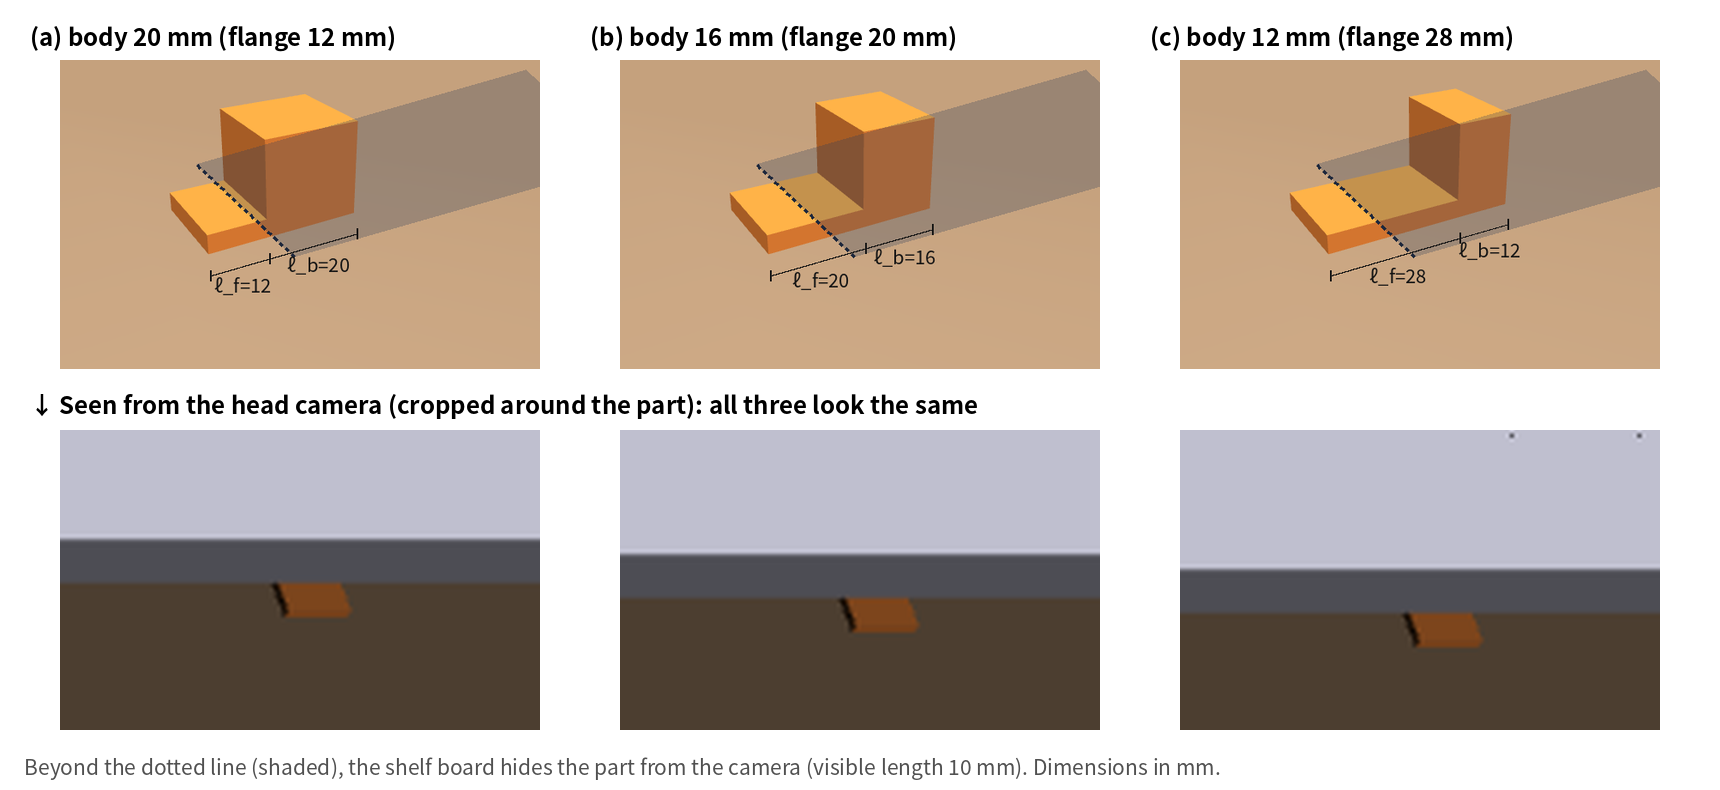
\includegraphics[width=\linewidth]{figures/shapes.png}
\caption{Shape family. Top: three parts with different flange and body lengths (MuJoCo rendering); the board hides everything beyond the dotted line. Bottom: the same layouts from the head camera. Only the front of the flange is visible and the three are indistinguishable, yet the place to pinch depends on where the body begins.}
\label{fig:shapes}
\end{figure}

\textbf{Observations.} The robot first obtains segmentation and depth from the head camera. A light touch at point $u$ from above returns one of four outcomes,
\begin{equation}
o\in\{\textsc{miss},\ \textsc{body-center},\ \textsc{body-other},\ \textsc{flange}\},
\end{equation}
where \textsc{body-center} means the fingertip center hit the body and \textsc{body-other} means another part of the finger (mostly the finger pad) hit it.

\textbf{Grasp and success.} A grasp moves the hand under the board above the grasp point $g$, pinches with the middle finger and thumb, pulls the part out, and lifts it. Success $S=1$ means the part is at least 4\,cm above its initial height after a 2\,s hold. Success depends on $\theta$, $g$, and unobserved physics $\xi$ (friction, mass, finger-control gain).

\textbf{Goal.} Choose touch points that maximize grasp success after $k$ touches; the main evaluation uses $k=1$.

\section{Method}

The belief over $\theta$ is a set of particles $\{\theta_i\}_{i=1}^{N}$, $N=200$, initialized from the camera and updated after each touch. Touch and grasp points are chosen from the particle-averaged success probability (Fig.~\ref{fig:pipeline}).

\begin{figure*}[t]
\centering
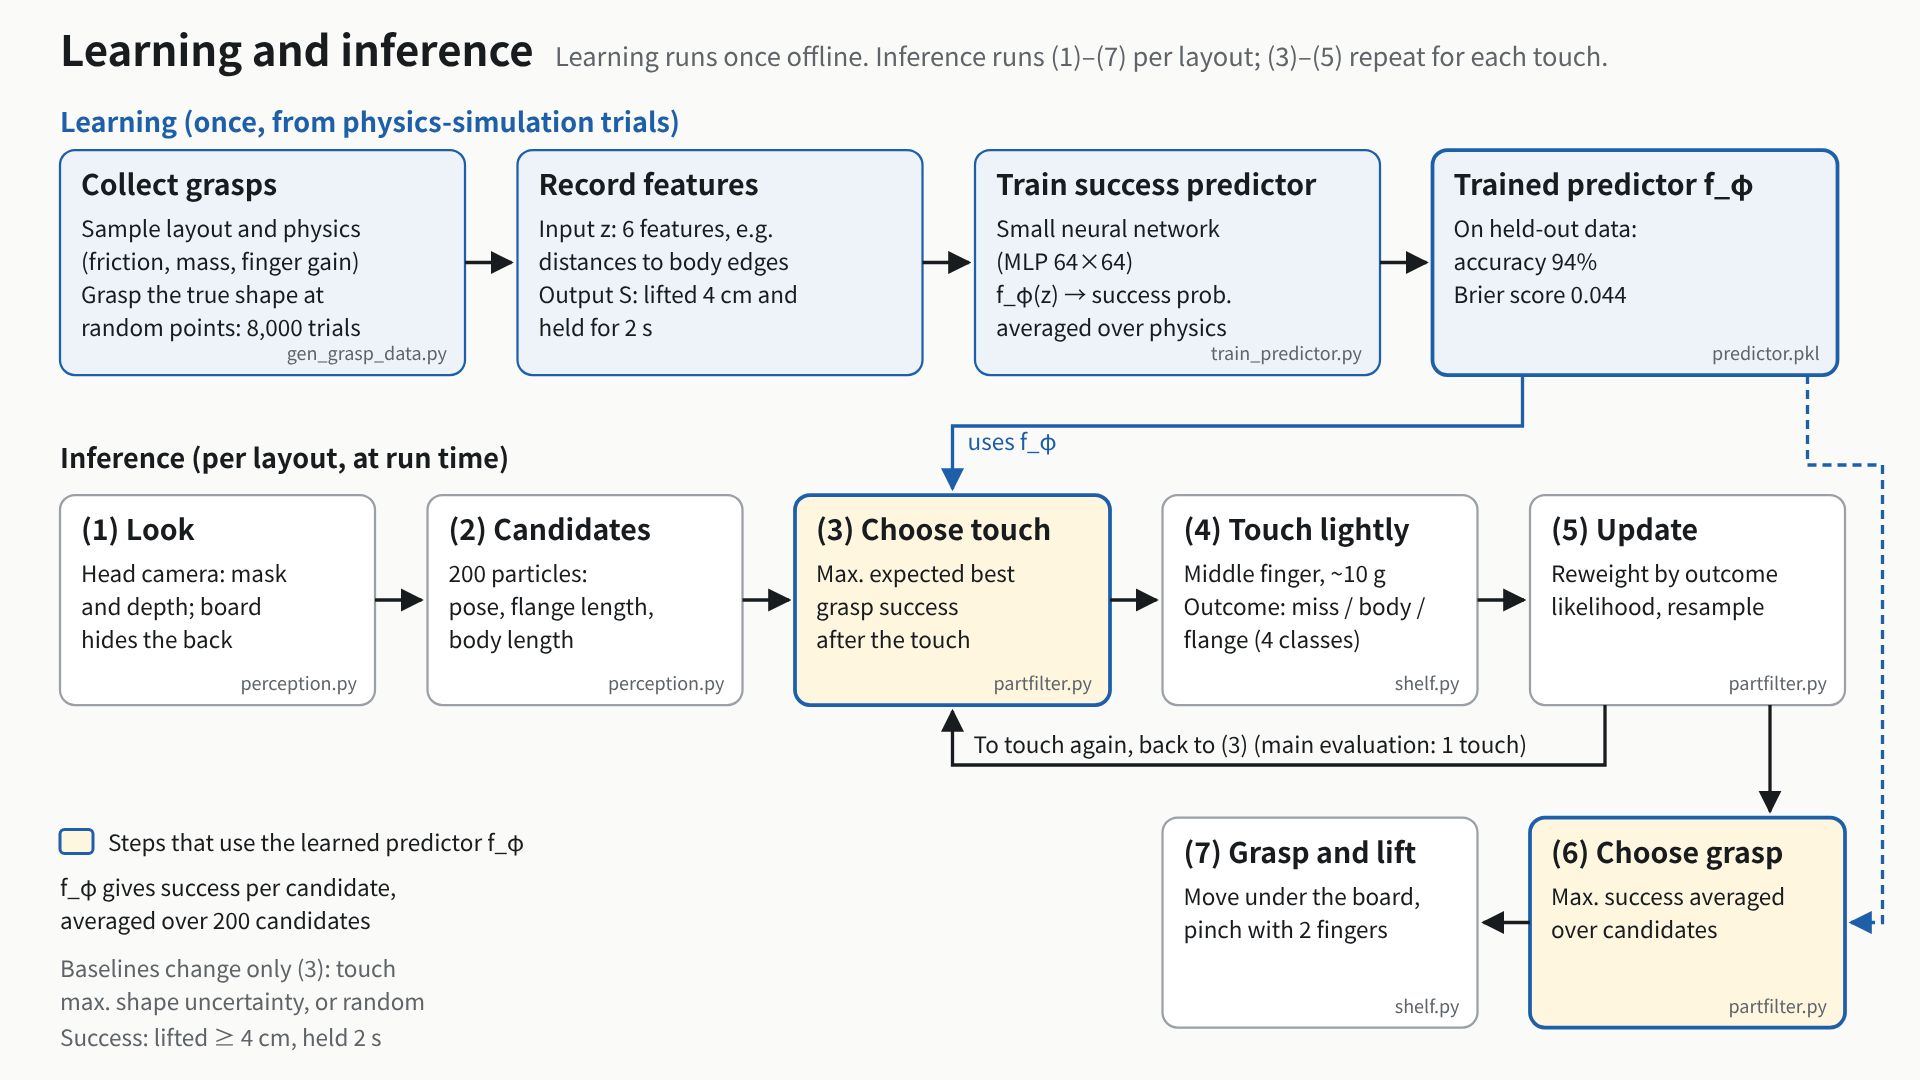
\includegraphics[width=0.92\textwidth]{figures/pipeline.png}
\caption{Learning and inference. Top: a success predictor $f_\phi$ is trained once from 8,000 simulated grasps (Sec.~\ref{sec:setup}). Bottom: per layout, the camera initializes 200 shape candidates (Sec.~\ref{sec:init}); the robot chooses a touch by the expected best success after the touch (Sec.~\ref{sec:touchsel}), touches, updates the candidates (Sec.~\ref{sec:obs}), and grasps at the point of highest averaged success (Sec.~\ref{sec:pred}). The baselines differ only in step (3). File names refer to the public code.}
\label{fig:pipeline}
\end{figure*}

\subsection{Initialization from the camera}\label{sec:init}
The part is about 20 pixels wide in the image, and errors at the segmentation boundary change the mask more than moderate changes of yaw or body position do. We therefore use depth in three ways.
(i) \emph{Yaw}: points at flange height (1.5--7\,mm above the table) are binned into 2\,mm lateral strips, the nearest point (5th percentile) of each strip is taken, and a line through them gives the front-edge direction (mean error 2.3$^\circ$, max 5.1$^\circ$ over 40 layouts).
(ii) \emph{Position}: 3,000 candidates are drawn around a prior; for each, the flange and body boxes are projected, the occluders in front (board, robot) are removed, and the expected visible region is compared with the observed mask, ignoring a one-pixel boundary. Weights $\exp(-(e-e_{\min})/T)$ with mismatch $e$ select 200 particles (mean front-face error 1.6\,mm).
(iii) \emph{Body}: if depth points higher than 10\,mm are found, the body is visible and $\ell_f$ is set from the nearest such point along the axis (30th percentile; within $\pm$1\,mm of the true edge). Otherwise the body must begin behind the line where a 10\,mm-high point starts to be hidden by the board, and $\ell_f$ is resampled uniformly beyond it. $\ell_b$ keeps its prior.

\subsection{Learned grasp success per shape candidate}\label{sec:pred}
A small multilayer perceptron $f_\phi$ predicts the success of pinching candidate $\theta$ at grasp point $g$. Its input $z(\theta,g)$ has six features: the distance from the body front edge to $g$, the distance from $g$ to the body back edge, the lateral offset, the yaw, the body length, and the depth of $g$ beyond the board front. The physics $\xi$ is not an input but is randomized in the training data, so $f_\phi$ approximates success averaged over $\xi$. Under belief $b$,
\begin{align}
P(S{=}1\mid g,b)&=\frac{1}{N}\sum_{i=1}^{N} f_\phi\bigl(z(\theta_i,g)\bigr),\\
g^*(b)&=\arg\max_{g\in G} P(S{=}1\mid g,b),
\end{align}
where $G$ are points every 1\,mm along the mean part axis.

\subsection{Touch observation model and update}\label{sec:obs}
Let $a$ be the axial and $c$ the lateral coordinate of $u$ for candidate $\theta$. The outcome depends on the distances to the body front edge $a-\ell_f$ and back edge $a-\ell_f-\ell_b$: up to $-11$\,mm in front of the front edge the finger lands on the flange; from $-11$ to $-3$\,mm the finger pad hits the body; from $-3$\,mm to 2\,mm past the back edge the fingertip center hits the body; from 2 to 12\,mm past the back edge the pad hits again; beyond that the touch misses. Nothing is hit if $|c|>W/2+3$\,mm. These boundaries were measured in preliminary trials; each is smoothed with a 1\,mm sigmoid, and every outcome keeps probability $\epsilon=0.02$. After a touch, particles are reweighted by $P(o\mid u,\theta_i)$, resampled, and jittered.

\subsection{Touch selection}\label{sec:touchsel}
For each candidate touch $u$, we compute the probability of each outcome and the best success after updating with that outcome, and pick
\begin{equation}
u^*=\arg\max_{u\in U}\sum_{o} P(o\mid u,b)\,\max_{g\in G} P(S{=}1\mid g,b_{u,o}),
\label{eq:voi}
\end{equation}
where $U$ are points every 3\,mm along the mean axis and $b_{u,o}$ is the belief after observing $o$ at $u$. The candidate-by-grasp success matrix is computed once; each $b_{u,o}$ only reweights its rows.

\textbf{Baselines.} \Unc{} (maximum shape uncertainty) touches where $p(u)(1-p(u))$ is largest, with $p(u)$ the fraction of particles whose body lies under $u$; this is the occupancy-variance criterion of Act-VH~\cite{rustler2022actvh} applied to our problem. \Rand{} chooses uniformly from $U$. \Geom{} uses the same lookahead (\ref{eq:voi}) and the same grasp choice, but replaces $f_\phi$ by a geometric tolerance: success if $g$ lies at least 3.5\,mm behind the body front edge, 2.5\,mm before the back edge, and within 5\,mm laterally (margins from preliminary grasps). \Geom{} is our closest analogue of DA-GRD's tolerance-based scoring.

\subsection{Touch motion}\label{sec:touchmotion}
A touch stops at about 10\,g so as not to move the part. With the wrist in the grasping orientation, the thumb is raised, and the middle fingertip descends from 1\,cm above the body top in 1\,mm steps until the contact force exceeds 0.1\,N. Reaching the table without touching the part is a miss. Outcomes are separated by whether the contact lies within 4\,mm of the fingertip center and by the contacted geometry (body or flange); on hardware we expect to use the contact location of a pressure sensor and the fingertip height at contact. After a touch, the fingertip returns to its start height and the arm stays under the board, moving horizontally to the next touch or grasp point.

\section{Experimental Setup}\label{sec:setup}

\begin{table}[t]
\caption{Simulation setup}
\label{tab:setup}
\centering
\small
\begin{tabular}{@{}p{0.22\linewidth}p{0.72\linewidth}@{}}
\toprule
Simulator & MuJoCo~\cite{todorov2012mujoco} 3.14, 2\,ms step, elliptic friction cone, impratio 10, torsional friction on the part \\
Robot & Unitree G1 with Dex3 (3 fingers) from MuJoCo Menagerie~\cite{menagerie2022}; pelvis fixed, whole-body gravity compensation \\
Grasp & Pinch with middle finger and thumb (index curled); IK by mink~\cite{zakka2024mink} on the 7 right-arm joints \\
Shelf & Table at 0.80\,m; board 20\,cm above it (1.5\,cm thick); part front face 31\,cm ahead and 25\,cm right of the robot \\
Camera & Head D435i-like camera, 640$\times$480; $\pm$1 pixel segmentation boundary errors; depth noise $\sigma(z)=z^2\cdot0.08/(f b)$ \\
Physics $\xi$ & Friction 0.3--1.0 (fingers and part), part mass $\pm$30\%, finger gain $\pm$20\%, drawn per layout \\
Layouts & $\ell_f,\ell_b$ uniform, yaw $\pm20^\circ$, lateral $\pm10$\,mm, $v$ cycling over 4 levels; fixed seeds shared by all rules \\
Predictor & 8,000 grasps on the true shape at random points; MLP 64$\times$64 (scikit-learn~\cite{pedregosa2011sklearn}); held-out accuracy 94\%, Brier 0.044 \\
\bottomrule
\end{tabular}
\end{table}

Table~\ref{tab:setup} lists the setup; Appendix~\ref{app:setup} gives the details. The shape ranges were set so that pinching the single best point without touching succeeds about 57\% of the time.

\textbf{Touch selection (main comparison).} For each of 240 layouts, each rule (\Ours, \Unc, \Rand, \Geom) touches up to twice, and the grasp at $g^*$ after each touch is recorded. Perception, predictor, and grasp selection are shared, except that \Geom{} uses the geometric tolerance for both touch and grasp choice.

\textbf{Number of touches and stopping.} On the first 120 layouts, \Ours{} touches up to four times and the grasp after each touch $k=0,\dots,4$ is recorded. From these we compute: no touch (A), $n$ touches (B$n$), and stopping at the first touch whose predicted success reaches $\tau$ (C($\tau$), at most four). Since the touch choice does not depend on $\tau$, this equals running each condition separately.

\textbf{Branching.} Each grasp is executed on a copy of the simulation state, and touching continues from the original state. Grasping twice from the same state gives identical results, and the copy matches grasping without copying.

\textbf{Metrics.} The main metric is grasp success after one touch. Differences are paired by layout, with 95\% bootstrap CIs (3,000 resamples over layouts) and McNemar's exact test on discordant layouts.

\section{Results}

\subsection{Where to touch}

\begin{figure}[t]
\centering
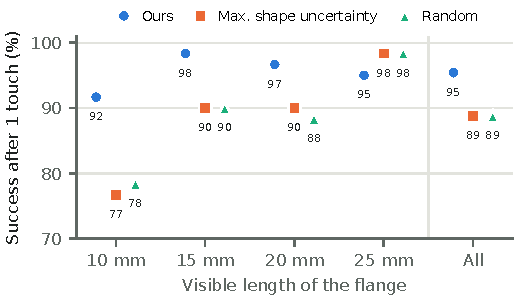
\includegraphics[width=\linewidth]{figures/success_by_vis.pdf}
\caption{Grasp success after one touch by visible length (240 layouts, 60 per level). \Geom{} uses the same lookahead as \Ours{} with a geometric tolerance instead of the learned success model.}
\label{fig:vis}
\end{figure}

After one touch, success was 95.4\% for \Ours, 88.8\% for \Unc, and 88.8\% for \Rand{} (Fig.~\ref{fig:vis}). The paired gain over \Unc{} was +6.7 points (95\% CI [+2.1, +11.3]; discordant layouts 23 vs.\ 7; McNemar $p=0.005$), and over \Rand{} also +6.7 ([+2.5, +11.3]; 23 vs.\ 7; $p=0.005$). The gain grew as less was visible: over \Unc{} it was +15.0 [+3.3, +26.7] at $v=10$\,mm, +8.3 [0.0, +16.7] at 15\,mm, +6.7 [0.0, +15.0] at 20\,mm, and $-3.3$ [$-8.3$, 0.0] at 25\,mm, where the body front edge is often visible to the camera.

After one touch, the median standard deviation of the body front edge estimate was 2.7\,mm (\Ours), 3.0\,mm (\Unc), and 3.1\,mm (\Rand): the difference in shape accuracy is small compared with the difference in grasp success. After two touches, success was 95.0\%, 91.7\%, and 88.3\%; the gap to \Unc{} shrank to +3.3 [0.0, +7.1] ($p=0.12$), because \Unc{} reaches the relevant region on its second touch.

\begin{figure*}[t]
\centering
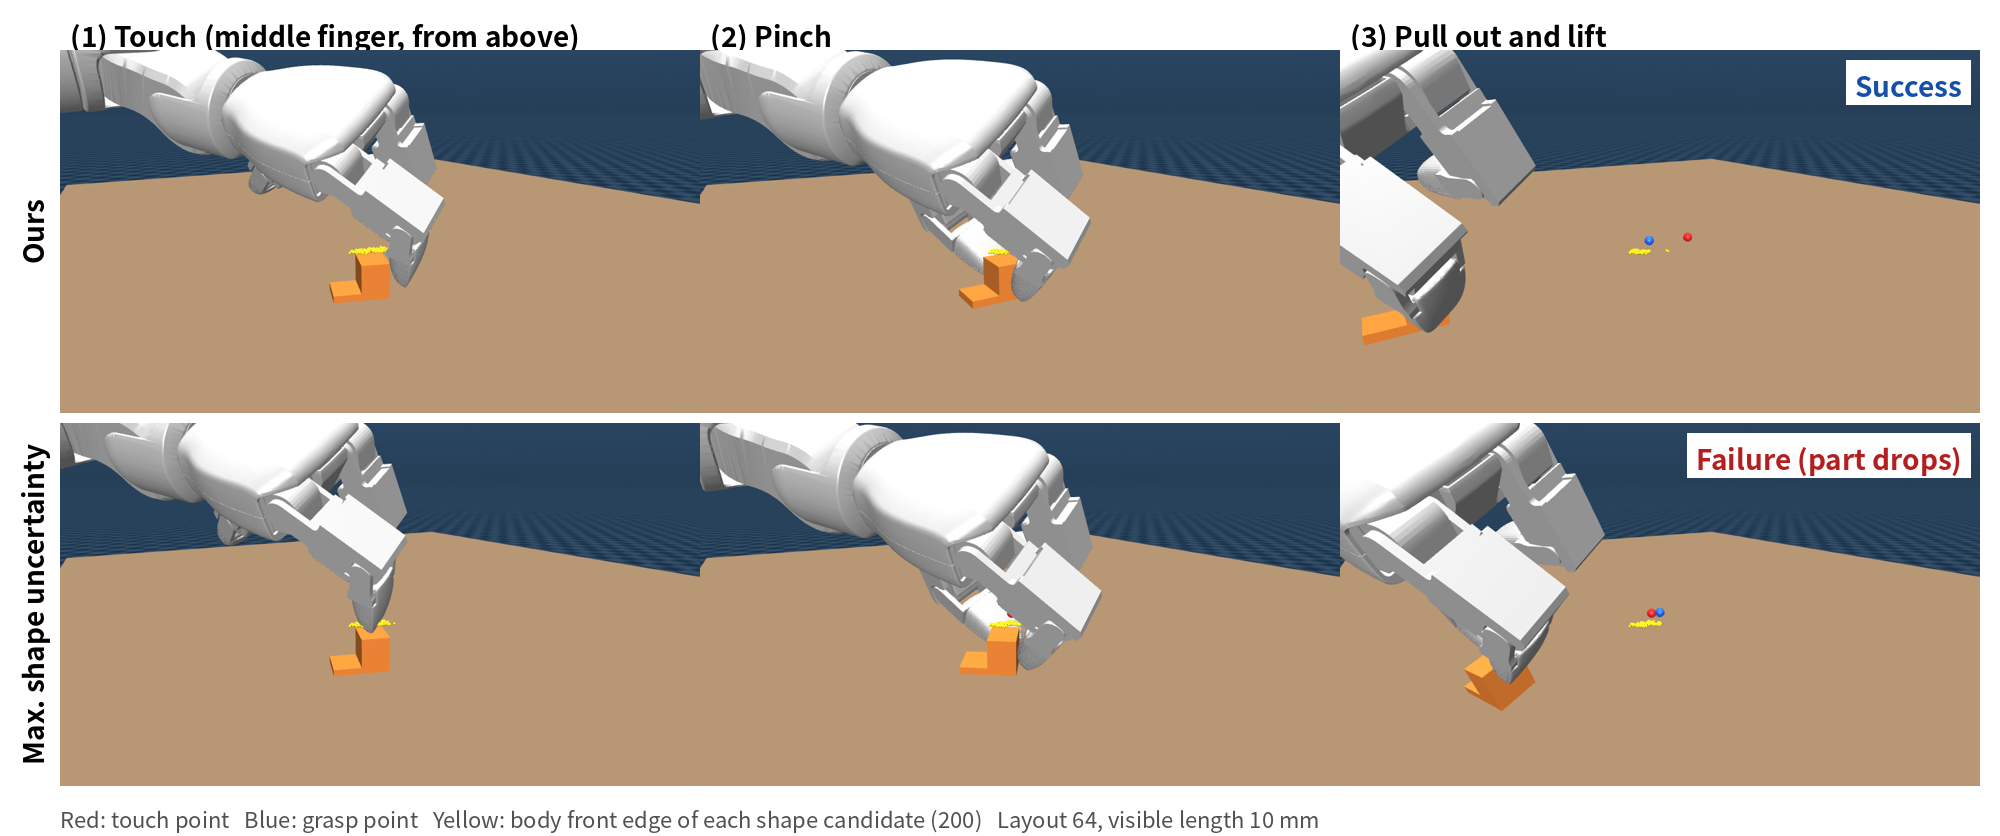
\includegraphics[width=0.95\textwidth]{figures/layout64.png}
\caption{Layout 64 ($v=10$\,mm; the body spans 15--31\,mm behind the front face). Top: \Ours{} touches 43\,mm behind the front face, beyond the body's far end, and misses. ``The body does not extend that far'' shrinks the spread of the body front edge from 5.9 to 2.9\,mm, and the grasp succeeds. Bottom: \Unc{} touches the middle of the body (23\,mm) and hits it, but the front edge keeps a 4.3\,mm spread (predicted success 0.63) and the grasp fails.}
\label{fig:layout64}
\end{figure*}

Fig.~\ref{fig:layout64} shows the difference in one layout. \Unc{} touches where the body ``may or may not be,'' which confirms that the body exists but says little about its front edge, which decides the grasp point. \Ours{} touches where the outcome changes the grasp choice most; here that was beyond the far end of the body, and the miss revealed that the body, and hence its front edge, lies further forward. Touching the far side is one example; in most layouts \Ours{} touches near the front edge (Sec.~\ref{sec:disc}).

\subsection{Learned versus geometric success}\label{sec:geom}
\GeomResultsParagraph{} The learned model therefore adds little to success in this setting: the grasp-centric lookahead, with either success model, is what separates the rules. Note that the geometric margins were measured with this hand in the same simulator; they are a strong baseline that the learned model must beat without any hand-measured tolerance.

\subsection{How many touches, and when to stop}

\begin{table}[t]
\caption{Number of touches and stopping (120 layouts)}
\label{tab:count}
\centering
\small
\begin{tabular}{@{}lccc@{}}
\toprule
Condition & Success & Touches & By $v$ = 10/15/20/25\,mm \\
\midrule
A: no touch & 72.5\% & 0 & 53 / 63 / 77 / 97\% \\
B1: 1 touch & 96.7\% & 1 & 90 / 100 / 97 / 100\% \\
B2: 2 touches & 94.2\% & 2 & 87 / 97 / 97 / 97\% \\
B3: 3 touches & 96.7\% & 3 & 97 / 97 / 100 / 93\% \\
C(0.85) & 95.0\% & 0.96 & 90 / 100 / 97 / 93\% \\
C(0.95) & 94.2\% & 1.61 & 93 / 100 / 97 / 87\% \\
\bottomrule
\end{tabular}
\end{table}

Without touching, success was 72.5\%, dropping to 53\% at $v=10$\,mm (Table~\ref{tab:count}). One touch raised it to 96.7\%, and more touches did not raise it further. The threshold rule C often skipped touching at $v=25$\,mm, but then failed slightly more often, and overall it did not beat B1 (C(0.85) minus B1: $-1.7$ points [$-4.2$, 0.0], $-0.04$ touches).

\subsection{Calibration}

\begin{figure}[t]
\centering
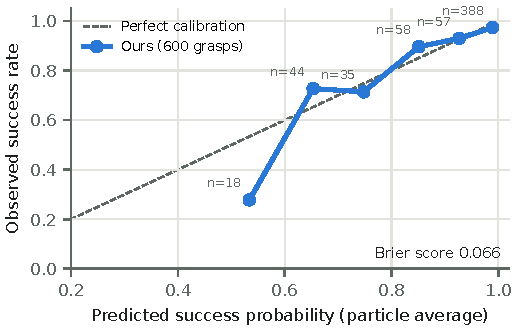
\includegraphics[width=0.95\linewidth]{figures/calibration.pdf}
\caption{Calibration of the particle-averaged success probability (120 layouts $\times$ 5 time points = 600 grasps).}
\label{fig:calib}
\end{figure}

The particle-averaged success probability matched the observed success rate well (Fig.~\ref{fig:calib}, Brier 0.066). Predictions $\ge0.9$ made up 74\% of grasps, with observed success of 93--97\%. Only the bin below 0.6 (18 grasps) was optimistic (28\% observed). On held-out training-distribution data the Brier score is 0.044, so the estimation errors in the full pipeline did not break the calibration. The training grasps approached from in front of the board without touching, yet the calibration held for grasps that start under the board after a touch.

\subsection{Cost of failure and time}\label{sec:cost}
Failed grasps moved the part substantially: in the 120 layouts, 91\% of 55 failures moved it by more than 10\,mm (median about 250\,mm), and in the 240 layouts, 98\% of 125 failures did (median about 140\,mm). The hand drags or flicks the part while pulling out. Pressing down during a touch moved the part by at most 0.33\,mm. Keeping the arm under the board after a touch, instead of retracting it and re-inserting, cut the median time to a completed grasp from 17.7 to 15.2\,s with one touch (about 14\%) and from 24.3 to 17.7\,s with two (about 27\%; 20 layouts, \Ours).

\section{Discussion and Limitations}\label{sec:disc}

\textbf{Why one touch suffices.} Success here is decided mainly by the position of the body front edge: the grasp point must be at least 3.5\,mm behind it and 2.5\,mm before the back edge. \Ours{} touches where the candidates split by outcome, i.e., around the body edges. Of its first touches, 59\% were outside the body (at least 3\,mm in front of the front edge or 5\,mm beyond the back edge) and only 5\% near the body middle; outcomes split into finger pad on body 46\%, fingertip center on body 38\%, flange 10\%, and miss 6\%. A pad or flange contact tells on which side of the edge the finger was. \Unc{} touched outside the body in only 18\% of layouts, and the fingertip center hit the body in 73\%: it confirms that the body is there but narrows little where the front edge is. This difference shows up much more in grasp success than in shape accuracy (2.7 vs.\ 3.0\,mm), which supports aiming exploration at the downstream grasp rather than at reconstruction.

One touch suffices because the depth profile of the part (front flange, body behind) is known and the unknown range is short. Once the camera fixes position and yaw, the remaining unknown is mostly the body front edge within about 20\,mm, while the graspable span inside the body is at least 6\,mm; one touch that tells which side of the edge it landed on is enough to place the grasp inside. Parts of unknown type or with longer unknown ranges may need more touches.

\textbf{What the learned model adds.} Under the same lookahead, the learned success model raised success by only \GeomDiffShort{} over the geometric tolerance (not significant) and gave a slightly lower Brier score. Two reasons are likely. The part family is simple: success is decided mostly by how far the grasp point lies inside the body edges, which a tolerance captures well. And the tolerance was itself measured in preliminary grasps with this hand in this simulator, so it already encodes most of what the physics trials teach. The learned model is still useful in two ways: it is obtained from physics trials without hand-measuring margins for each new hand or part, and it gives probabilities that can be compared with a threshold or across actions. Whether it pays off more for parts whose success depends on friction, mass distribution, or contact geometry in ways a tolerance cannot express is open.

\textbf{Why stopping did not help.} One well-chosen touch already brings success near its ceiling (about 97\%), and most remaining failures come from unobserved physics such as friction. When outcomes are only hit/miss or more quantities are unknown, stopping could save touches without losing success; we did not test this.

\textbf{Touching moves the part.} The estimator assumes a static part. In an early implementation the finger dragged the part by about 1\,mm while withdrawing after each touch, and errors accumulated with more touches. Withdrawing straight up in fine steps and never lowering the finger under the board reduced the motion during touching to at most 0.33\,mm. Modeling part motion in the estimator is future work.

\textbf{The conclusion does not depend on the arm motion.} With the initial motion, which retracted the arm out from under the board after every touch, the same experiment gave 95.8\% (\Ours), 90.0\% (\Unc), and 88.3\% (\Rand) after one touch (+5.8 [+1.7, +9.6], $p=0.007$ over \Unc); no touch gave 72.5\% and one touch 95.8\% (Appendix~\ref{app:v1}).

\textbf{Limitations.} First, all results are in simulation. The observation boundaries and grasp tolerances depend on the simulated finger geometry and contact model, and real pressure sensing and friction may fall outside the randomized ranges. Second, the shape type is known with two unknown lengths; other part types need candidates from a CAD-based family or from neural shape completion~\cite{rustler2022actvh,rustler2026shapegrasp}. The touch-selection rule does not depend on how candidates are represented. Third, \Unc{} re-implements the Act-VH criterion for our problem and is not the original method. Fourth, touch candidates lie on a one-dimensional axis. Fifth, the hand path and finger opening are scripted: fixed waypoints solved by inverse kinematics. Only the touch and grasp points are decided by learning and inference, so the rules differ only in where they touch, and differences in success come from that choice alone. On the other hand, we do not plan paths around the board or neighboring objects, and on hardware, joint tracking lag and lower fingertip friction could make the same scripted motion fail more often; slowing it down would reduce this at the cost of the time savings above.

\section{Conclusion}

To grasp a part whose back is hidden by a shelf board, we choose where to touch by the expected best grasp success after the touch, averaged over shape candidates. On 240 paired layouts, one touch chosen this way gave 95.4\% grasp success, against 88.8\% for touching at the largest shape uncertainty and 88.8\% for random touches, with the largest gain when the least was visible. A geometric tolerance in place of the learned success model gave \GeomSucc, so the criterion matters more than the success model in this setting. When touch is used to complete a shape, the robot should touch where the outcome changes the grasp choice most, not where the shape could be reconstructed best. Hardware validation, broader shape families, and modeling part motion during touching remain future work.

\bibliographystyle{IEEEtran}
\bibliography{refs}

\appendix
% Appendix: details for reproduction. Section labels are referenced from main.tex.

\section{Setup details}\label{app:setup}

\textbf{Scene.} The G1 model with Dex3 hands is taken from MuJoCo Menagerie~\cite{menagerie2022} at commit \texttt{c96a32d}. The pelvis is fixed to the world, gravity compensation is applied to the whole body (compensating only the right arm let the waist sag by about 4$^\circ$, which tilted the head camera), and the left arm is moved off the table. The head camera follows the D435i mount of the Unitree URDF (pitched about 48$^\circ$ down, vertical field of view 58$^\circ$). The part is one rigid body of two boxes (density 600\,kg/m$^3$, torsional friction enabled with \texttt{condim}=4); the flange box overlaps the body by 1\,mm.

\textbf{Visibility.} For a visible length $v$, the board front is placed so that the ray from the head camera through the lower front edge of the board meets the flange top surface $v$ behind the part's front face.

\textbf{Grasp motion.} The wrist is rolled $-60^\circ$, pitched $10^\circ$, and yawed $-55^\circ$ about the vertical, so that the pinch axis is almost lateral; the index finger is curled. Without a previous touch, the hand is inserted horizontally from 10\,cm in front of the board at 20\,mm above the grasp point, then lowered. After a touch, the hand moves under the board at or above its current height to above the grasp point. The thumb and middle finger close independently, each stopping at contact; once both touch, both close a further fixed amount over 0.3\,s. The hand then raises the part by 1\,cm, pulls it out to 10\,cm in front of the board, lifts it to 6\,cm above the grasp height, and holds for 2\,s. Moves near and under the board are straight lines in Cartesian space split into waypoints (15 by default; one per 1\,mm step during the touch descent and 12 for the withdrawal), each solved by mink~\cite{zakka2024mink}, with joint targets interpolated linearly in time. Moves in free space (the approach in front of the board and wrist re-orientation) solve inverse kinematics once and interpolate in joint space.

\textbf{Physics randomization.} Per layout: friction coefficient $\mu\sim U[0.3,1.0]$ on the fingers and the part (MuJoCo uses the larger of two contacting geoms), part mass and inertia scaled by $U[0.7,1.3]$, and the position gains of the hand actuators scaled by $U[0.8,1.2]$. MuJoCo's derived constants are recomputed after changing the mass; otherwise the simulation becomes unstable and success drops spuriously.

\textbf{Camera model.} Segmentation is the simulator's ground truth, corrupted by eroding or dilating the mask by one pixel (probability 1/3 each, otherwise unchanged) and flipping 30\% of the boundary pixels. Depth noise follows the D435i model $\sigma(z)=z^2\cdot0.08/(f b)$ with baseline $b=50$\,mm.

\textbf{Particle filter.} 3,000 prior candidates: front-face position $\mathcal{N}(\text{prior},\,(30\,\text{mm})^2)$ in depth and $\mathcal{N}(\text{prior},\,(15\,\text{mm})^2)$ laterally, yaw $\mathcal{N}(\hat\psi,\,(3.5^\circ)^2)$ around the depth-based estimate, $\ell_f\sim U[10,30]$\,mm, $\ell_b\sim U[12,20]$\,mm. Matching temperature $T=0.05$. 200 particles are drawn with jitter (0.5\,mm, 1$^\circ$). After each touch, particles are resampled with jitter (0.3\,mm, 0.5$^\circ$). Grasp candidates lie every 1\,mm and touch candidates every 3\,mm, from 0 to 55\,mm behind the mean front face.

\textbf{Predictor training.} Each of the 8,000 training grasps draws a layout as above and pinches the true shape at axial position $a\sim U[\ell_f-6\,\text{mm},\ \ell_f+\ell_b+4\,\text{mm}]$, lateral offset $U[-8,8]$\,mm, and a height error of $\mathcal{N}(0,(1\,\text{mm})^2)$. The overall success rate was 48\%. The MLP has two hidden layers of 64 units ($\alpha=10^{-3}$, early stopping) on standardized features in millimeters and degrees. Trained on the first 80\% and tested on the last 20\% (1,600 grasps), accuracy was 0.943 and the Brier score 0.044; the released model is retrained on all 8,000 grasps.

\textbf{Touch observation boundaries.} With $d_f=a-\ell_f$ and $d_b=a-\ell_f-\ell_b$: \textsc{flange} for $a\ge0$ and $d_f<-11$\,mm; \textsc{body-other} for $-11\le d_f<-3$\,mm; \textsc{body-center} for $d_f\ge-3$\,mm and $d_b<2$\,mm; \textsc{body-other} for $2\le d_b<12$\,mm; \textsc{miss} otherwise or when the lateral offset exceeds $W/2+3$\,mm. In the simulator, \textsc{body-center} is a body contact within 4\,mm of the fingertip center, and a touch stops at 0.1\,N.

\section{Results with the initial arm motion}\label{app:v1}
The initial implementation retracted the arm out from under the board after every touch, re-inserted it, and returned the thumb to the grasping posture immediately. With that motion, success after one touch was 95.8\% (\Ours), 90.0\% (\Unc), and 88.3\% (\Rand); the paired gain over \Unc{} was +5.8 points [+1.7, +9.6] ($p=0.007$). In the touch-count experiment, no touch gave 72.5\% and one touch 95.8\%. Both sets of raw results are in the repository (\texttt{results/v1\_retract/}). In a separate timing run on 20 layouts (not stored), the initial motion took a median of 17.7\,s with one touch and 24.3\,s with two, against 15.2\,s and 17.7\,s for the motion used in the paper.

\section{Combining with a vision-language model}\label{app:vlm}
Our method decides where to touch and where to pinch, not which part to pick. We combined it with SmolVLM~\cite{marafioti2025smolvlm}, which picks the part from an instruction. Two parts that differ in color and in hidden size are placed 10\,cm apart under the board (at 5\,cm the hand hit the neighbor). Since the board front is shared, both show the same length of flange to the camera, and the size difference is invisible. SmolVLM-500M receives the head-camera image, cropped and enlarged with numbers drawn above the parts, and an English instruction (e.g., ``Pick up the green part.''), and answers with a number; the chosen part is then touched and grasped by our method. In three runs on the author's GPU, including a different color in the instruction and swapped positions, SmolVLM-500M chose the correct part and the robot lifted it.

\begin{figure*}[t]
\centering
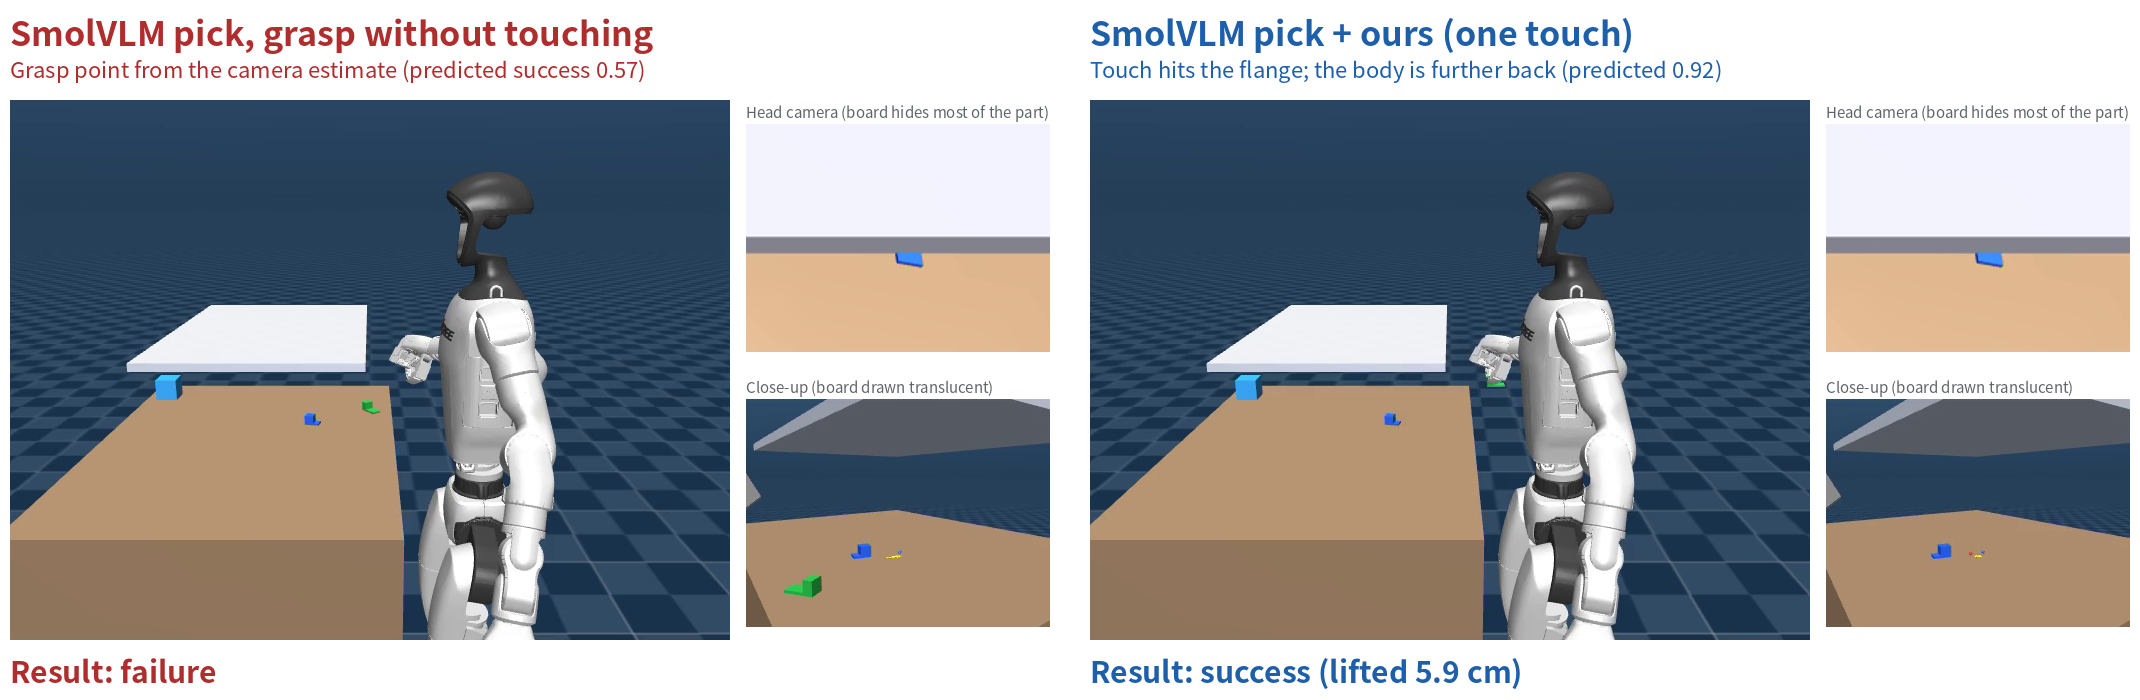
\includegraphics[width=0.95\textwidth]{figures/vlm_compare.png}
\caption{Same scene, same SmolVLM answer (``2'', the green part: flange 28\,mm, body 13\,mm). Left: grasping from the camera estimate without touching fails. Right: one touch lands on the flange, revealing that the body lies further back, and the grasp succeeds. The arm motion is identical; only the touch differs.}
\label{fig:vlm}
\end{figure*}

We then compared how to grasp the chosen part on 60 layouts $\times$ 2 parts = 120 trials (hidden sizes drawn from the predictor's training ranges; other settings as in Sec.~\ref{sec:setup}). All conditions are evaluated from the same observation by branching, and the part choice is assumed correct. For the VLM-grasp conditions, six candidate points A--F (8--48\,mm behind the estimated front face, every 8\,mm) are drawn on the image and SmolVLM chooses one zero-shot.

\begin{table}[h]
\caption{Choosing the grasp point for the picked part (120 trials)}
\label{tab:vlm}
\centering
\small
\begin{tabular}{@{}lc@{}}
\toprule
Grasp point chosen by & Success \\
\midrule
SmolVLM-500M, no part knowledge & 0.8\% \\
SmolVLM-2.2B, no part knowledge & 0.8\% \\
SmolVLM-500M, length ranges given in text & 43.3\% \\
SmolVLM-2.2B, length ranges given in text & 61.7\% \\
Learned predictor, no touch & 75.8\% \\
Ours, one touch & 95.0\% \\
\bottomrule
\end{tabular}
\end{table}

Without part knowledge, SmolVLM-500M answered only A or F and SmolVLM-2.2B only F, and almost nothing was lifted. Given the flange and body length ranges, the candidate distances, and the required margin in text, the models chose middle points, but SmolVLM-2.2B answered only C or D, comparable to always choosing C (57\%) or D (65\%). The body is hidden by the board, so the image offers no cue for moving the grasp point per layout. The learned predictor, which uses the same camera estimate, reached 75.8\%, 14.2 points above SmolVLM-2.2B (discordant 32 vs.\ 15, McNemar $p=0.019$). One touch raised success to 95.0\%, 19.2 points above the predictor without touching (95\% CI [+11.7, +26.7]; discordant 25 vs.\ 2; $p<0.001$); at $v=10$\,mm it rose from 63\% to 93\%. Both prompts are given verbatim in \texttt{run\_vlm\_point.py}.

\section{Reproduction}\label{app:repro}
Code, the trained predictor, all raw results, and videos are at \url{https://github.com/Nishina-N/Physics-Informed-Touch-Selection}. The environment is Python 3.11 with MuJoCo 3.14, mink 1.3, and scikit-learn 1.8.0 (locked in \texttt{uv.lock}).
\begin{footnotesize}
\begin{verbatim}
uv sync
git clone https://github.com/google-deepmind/\
mujoco_menagerie third_party/mujoco_menagerie
git -C third_party/mujoco_menagerie checkout \
  c96a32d28fb5da84da38c1da4d749e7a13212855
# numbers from the stored results (seconds)
uv run python analyze_touchsel.py
uv run python analyze_branch.py
# retrain the predictor (seconds)
uv run python train_predictor.py
# rerun everything (k = 0..n-1 in parallel)
uv run python gen_grasp_data.py 0 2 8000
uv run python run_touchsel.py 0 2 240 predictor.pkl
TSEL_RULES=geom uv run python run_touchsel.py \
  0 2 240 predictor.pkl
uv run python run_branch.py 0 2 120 predictor.pkl
\end{verbatim}
\end{footnotesize}
Expected outputs: \texttt{analyze\_touchsel.py} prints success 0.954 (\Ours), 0.887 (\Unc; 213/240 = 88.75\%, reported as 88.8\%), and a paired difference of +0.067 with McNemar $p=0.005$; \texttt{analyze\_branch.py} prints 0.725 for A, 0.967 for B1, and the C(0.85)$-$B1 difference; \texttt{paper/make\_numbers.py} and \texttt{paper/make\_figures.py} regenerate the ablation numbers and result figures; \texttt{train\_predictor.py} prints Brier 0.044 and accuracy 0.943 and reproduces \texttt{predictor.pkl}. Layouts are fixed by seeds, so a rerun of layout 0 reproduces the stored result exactly. On one CPU core, generating the training data takes about 3.5\,h, and the 120-layout touch-count experiment about 20\,min. \texttt{view\_trial.py 64 --rule voi} shows the trial of Fig.~\ref{fig:layout64}, and \texttt{docs/code\_guide.html} walks through the code in execution order.


\end{document}
